\documentclass[border=10pt]{standalone}
\usepackage{amsmath}
\usepackage{amssymb}
\usepackage{tikz}
\usetikzlibrary{arrows.meta,calc,decorations.pathreplacing,decorations.pathmorphing,patterns,shapes.geometric,positioning,shadings,plotmarks}

\begin{document}
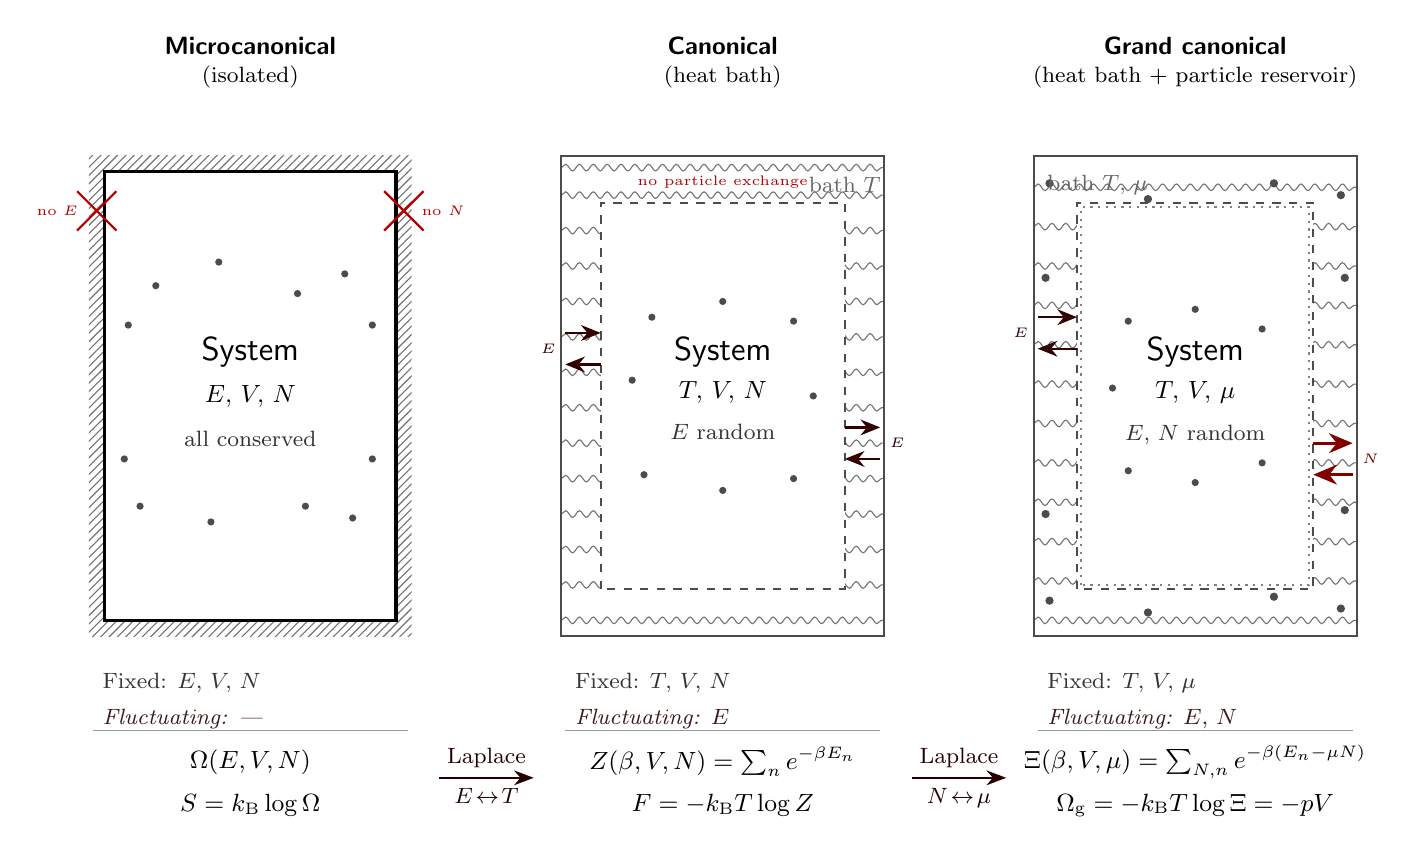
\begin{tikzpicture}[
  font=\sffamily,
  every node/.style={transform shape},
  accent/.style={color=black!85!red!90, thick},
  fixed/.style={very thick, draw=black},
  open/.style={thick, dashed, draw=black!70},
  energybath/.style={decorate, decoration={snake, amplitude=1.2pt, segment length=5pt}, draw=black!55},
  particlebath/.style={draw=black!50, dotted, thick},
  arrowE/.style={-{Stealth[length=2.5mm,width=2mm]}, thick, black!80!red},
  arrowN/.style={-{Stealth[length=3mm,width=2.5mm]}, very thick, black!50!red},
  panellabel/.style={font=\small\sffamily\bfseries},
  formula/.style={font=\small},
  fluct/.style={font=\footnotesize\itshape, color=black!85!red!90},
  fixedlabel/.style={font=\footnotesize, color=black!80}
]

% ============== panel parameters ==============
\def\panelw{4.4}     % half width
\def\panelh{3.0}     % box half-height (visible inner box)
\def\xA{0}
\def\xB{6.0}
\def\xC{12.0}

% ===========================================================
% PANEL A: Microcanonical -- isolated, rigid adiabatic walls
% ===========================================================
\node[panellabel] at (\xA, \panelh+1.45) {Microcanonical};
\node[font=\footnotesize] at (\xA, \panelh+1.05) {(isolated)};

% Hatched outer frame indicating thick adiabatic rigid walls
\fill[pattern=north east lines, pattern color=black!55]
  (\xA-2.05,-\panelh-0.05) rectangle (\xA+2.05, \panelh+0.05);
\fill[white]
  (\xA-1.85,-\panelh+0.15) rectangle (\xA+1.85, \panelh-0.15);

% Inner system box (sealed)
\draw[fixed] (\xA-1.85,-\panelh+0.15) rectangle (\xA+1.85, \panelh-0.15);

% System contents
\node at (\xA, 0.55) {\large System};
\node[formula] at (\xA, 0.0) {$E,\, V,\, N$};
\node[fixedlabel] at (\xA, -0.55) {all conserved};

% Decorative dots representing particles inside
\foreach \p in {(-1.2,1.4),(-0.4,1.7),(0.6,1.3),(1.2,1.55),
                (-1.4,-1.4),(-0.5,-1.6),(0.7,-1.4),(1.3,-1.55),
                (-1.55,0.9),(1.55,0.9),(-1.6,-0.8),(1.55,-0.8)}{
  \fill[black!70] \p ++(\xA, 0) circle (1.3pt);
}

% No-exchange indicator
\draw[red!70!black, thick] (\xA-2.2, \panelh-0.4) -- (\xA-1.7, \panelh-0.9);
\draw[red!70!black, thick] (\xA-2.2, \panelh-0.9) -- (\xA-1.7, \panelh-0.4);
\node[font=\tiny, red!70!black] at (\xA-2.45, \panelh-0.65) {no $E$};

\draw[red!70!black, thick] (\xA+1.7, \panelh-0.4) -- (\xA+2.2, \panelh-0.9);
\draw[red!70!black, thick] (\xA+1.7, \panelh-0.9) -- (\xA+2.2, \panelh-0.4);
\node[font=\tiny, red!70!black] at (\xA+2.45, \panelh-0.65) {no $N$};

% Fixed/Fluctuating tags
\node[fixedlabel, anchor=north west] at (\xA-2.0, -\panelh-0.4) {Fixed: $E,\,V,\,N$};
\node[fluct, anchor=north west]      at (\xA-2.0, -\panelh-0.85) {Fluctuating: ---};

% Formula below
\draw[black!40, thin] (\xA-2.0,-\panelh-1.25) -- (\xA+2.0,-\panelh-1.25);
\node[formula] at (\xA, -\panelh-1.65) {$\Omega(E,V,N)$};
\node[formula] at (\xA, -\panelh-2.20) {$S = k_{\mathrm B}\log\Omega$};

% ===========================================================
% PANEL B: Canonical -- in heat bath
% ===========================================================
\node[panellabel] at (\xB, \panelh+1.45) {Canonical};
\node[font=\footnotesize] at (\xB, \panelh+1.05) {(heat bath)};

% Outer "heat bath" wavy region (horizontal wavy lines)
\begin{scope}
  \clip (\xB-2.05,-\panelh-0.05) rectangle (\xB+2.05, \panelh+0.05);
  \foreach \y in {-2.85,-2.4,-1.95,-1.5,-1.05,-0.6,-0.15,0.3,0.75,1.2,1.65,2.1,2.55,2.9}{
    \draw[energybath] (\xB-2.05, \y) -- (\xB+2.05, \y);
  }
\end{scope}
\draw[black!70, thick] (\xB-2.05,-\panelh-0.05) rectangle (\xB+2.05, \panelh+0.05);
\node[font=\footnotesize, black!60] at (\xB+1.55, \panelh-0.32) {bath $T$};

% Inner system box -- diathermal walls (dashed) but rigid+impermeable to N
\fill[white] (\xB-1.55,-\panelh+0.55) rectangle (\xB+1.55, \panelh-0.55);
\draw[open] (\xB-1.55,-\panelh+0.55) rectangle (\xB+1.55, \panelh-0.55);

\node at (\xB, 0.55) {\large System};
\node[formula] at (\xB, 0.05) {$T,\, V,\, N$};
\node[fixedlabel] at (\xB, -0.45) {$E$ random};

% Particles
\foreach \p in {(-0.9,1.0),(0.0,1.2),(0.9,0.95),
                (-1.0,-1.0),(0.0,-1.2),(0.9,-1.05),
                (-1.15,0.2),(1.15,0.0)}{
  \fill[black!70] \p ++(\xB, 0) circle (1.3pt);
}

% Two-way energy arrows (across left and right walls)
\draw[arrowE] (\xB-2.0, 0.8) -- (\xB-1.55, 0.8);
\draw[arrowE] (\xB-1.55, 0.4) -- (\xB-2.0, 0.4);
\node[font=\tiny, color=black!80!red, anchor=east] at (\xB-2.0, 0.6) {$E$};

\draw[arrowE] (\xB+1.55, -0.4) -- (\xB+2.0, -0.4);
\draw[arrowE] (\xB+2.0, -0.8) -- (\xB+1.55, -0.8);
\node[font=\tiny, color=black!80!red, anchor=west] at (\xB+2.0, -0.6) {$E$};

% No-N indicator
\node[font=\tiny, red!70!black] at (\xB, \panelh-0.28) {no particle exchange};

% Fixed/Fluctuating tags
\node[fixedlabel, anchor=north west] at (\xB-2.0, -\panelh-0.4) {Fixed: $T,\,V,\,N$};
\node[fluct, anchor=north west]      at (\xB-2.0, -\panelh-0.85) {Fluctuating: $E$};

\draw[black!40, thin] (\xB-2.0,-\panelh-1.25) -- (\xB+2.0,-\panelh-1.25);
\node[formula] at (\xB, -\panelh-1.65) {$Z(\beta,V,N) = \sum_n e^{-\beta E_n}$};
\node[formula] at (\xB, -\panelh-2.20) {$F = -k_{\mathrm B}T\log Z$};

% ===========================================================
% PANEL C: Grand canonical -- heat + particle reservoir
% ===========================================================
\node[panellabel] at (\xC, \panelh+1.45) {Grand canonical};
\node[font=\footnotesize] at (\xC, \panelh+1.05) {(heat bath $+$ particle reservoir)};

% Outer environment region: heat bath wavy + particle dots
\begin{scope}
  \clip (\xC-2.05,-\panelh-0.05) rectangle (\xC+2.05, \panelh+0.05);
  \foreach \y in {-2.85,-2.35,-1.85,-1.35,-0.85,-0.35,0.15,0.65,1.15,1.65,2.15,2.65}{
    \draw[energybath] (\xC-2.05, \y) -- (\xC+2.05, \y);
  }
  \foreach \p in {(-1.85,2.7),(-0.6,2.5),(1.0,2.7),(1.85,2.55),
                  (-1.85,-2.6),(-0.6,-2.75),(1.0,-2.55),(1.85,-2.7),
                  (-1.9,1.5),(1.9,-1.45),(-1.9,-1.5),(1.9,1.5)}{
    \fill[black!70] \p ++(\xC, 0) circle (1.5pt);
  }
\end{scope}
\draw[black!70, thick] (\xC-2.05,-\panelh-0.05) rectangle (\xC+2.05, \panelh+0.05);
\node[font=\footnotesize, black!60, anchor=west] at (\xC-2.0, \panelh-0.32) {bath $T$, $\mu$};

% Inner system box -- both diathermal AND permeable (dashed + dotted)
\fill[white] (\xC-1.5,-\panelh+0.55) rectangle (\xC+1.5, \panelh-0.55);
\draw[open] (\xC-1.5,-\panelh+0.55) rectangle (\xC+1.5, \panelh-0.55);
\draw[particlebath] (\xC-1.45,-\panelh+0.6) rectangle (\xC+1.45, \panelh-0.6);

\node at (\xC, 0.55) {\large System};
\node[formula] at (\xC, 0.05) {$T,\, V,\, \mu$};
\node[fixedlabel] at (\xC, -0.5) {$E,\,N$ random};

% Particles inside (varying number)
\foreach \p in {(-0.85,0.95),(0.0,1.1),(0.85,0.85),
                (-0.85,-0.95),(0.0,-1.1),(0.85,-0.85),
                (-1.05,0.1)}{
  \fill[black!70] \p ++(\xC, 0) circle (1.3pt);
}

% Energy arrows (thin)
\draw[arrowE] (\xC-2.0, 1.0) -- (\xC-1.5, 1.0);
\draw[arrowE] (\xC-1.5, 0.6) -- (\xC-2.0, 0.6);
\node[font=\tiny, color=black!80!red, anchor=east] at (\xC-2.0, 0.8) {$E$};

% Particle arrows (thicker)
\draw[arrowN] (\xC+1.5, -0.6) -- (\xC+2.0, -0.6);
\draw[arrowN] (\xC+2.0, -1.0) -- (\xC+1.5, -1.0);
\node[font=\tiny, color=black!50!red, anchor=west] at (\xC+2.0, -0.8) {$N$};

% Fixed/Fluctuating tags
\node[fixedlabel, anchor=north west] at (\xC-2.0, -\panelh-0.4) {Fixed: $T,\,V,\,\mu$};
\node[fluct, anchor=north west]      at (\xC-2.0, -\panelh-0.85) {Fluctuating: $E,\,N$};

\draw[black!40, thin] (\xC-2.0,-\panelh-1.25) -- (\xC+2.0,-\panelh-1.25);
\node[formula] at (\xC, -\panelh-1.65) {$\Xi(\beta,V,\mu) = \sum_{N,n} e^{-\beta(E_n-\mu N)}$};
\node[formula] at (\xC, -\panelh-2.20) {$\Omega_{\mathrm g} = -k_{\mathrm B}T\log\Xi = -pV$};

% ===========================================================
% Bottom: Legendre / Laplace chain connecting them
% ===========================================================
\draw[-{Stealth[length=2.5mm]}, thick, black!85!red] (\xA+2.4, -\panelh-1.85) -- (\xB-2.4, -\panelh-1.85)
  node[midway, above, font=\footnotesize] {Laplace}
  node[midway, below, font=\footnotesize] {$E\!\leftrightarrow\!T$};
\draw[-{Stealth[length=2.5mm]}, thick, black!85!red] (\xB+2.4, -\panelh-1.85) -- (\xC-2.4, -\panelh-1.85)
  node[midway, above, font=\footnotesize] {Laplace}
  node[midway, below, font=\footnotesize] {$N\!\leftrightarrow\!\mu$};

\end{tikzpicture}
\end{document}
